\doublespacing
\section*{General Introduction}
\subsection*{The electricity markets and their modelization over time}
\subsubsection*{Public utility pricing}

The interest for modelling the electricity markets can be traced back to the reference work by Marcel Boiteux, vice president in charge of economic studies at Electricité de France, at the outset of the second world war. The question at the time was mainly that of public utility pricing: in the context of a public monopoly, which price should the consumers face in order to allow the producers to recover their costs. \\

There are two main concerns that electricity producers have to face: the uncertainty of demand and the cyclicity of demand, for a commodity that essentially cannot be stored.\footnote{Electricity can be stored in hydroelectric dams, but the total energy stored is not enough to stabilize completely the demand faced by the other generation units, and only a fraction of the hydroelectric storage capacities can be actively replenished: the pumped storage facilities, which have two lakes and can therefore pump from the lower lake to the upper one on demand to store more electricity that that naturally stored in a lake that would be naturally replenished by a river.} \\

The first question is addressed in \cite{boiteux1951tarification}. In this paper, Boiteux considers a constant expected demand with fluctuations. The goal is to find the correct marginal pricing so that consumers internalize the additional cost that an uncertain demand entails for the producer. With a certain probability that demand is above its expected value by a given amount, how much more reserve capacity has to be kept in order to insure an accepted failure probability.\footnote{In the context of electricity, as production has to match demand at every point in time, every national grid is built with the notion of an acceptable probability of mismatch which translates in curtailments}\\

The second question is addressed in \cite{boiteux1960peak}. Contrary to the previous situation, demand is now considered to change over time in a deterministic and cyclical fashion. The question is to price electricity in order for consumers to be sensitive to the additional investment cost implied by higher demand peaks. \\

These contributions have sparked a larger litterature on the question of the pricing of economically non-storable commodities whose demand varies periodically, first in \cite{brown1969public} which studies the impact of stochastic demand on expected welfare. We refer the interested reader to the following review \cite{crew1995theory}. \\ 

This litterature has been mainly interested in questions of optimal pricing when the agent choosing the pricing tries to maximize the consumer's welfare, that is in the case of public monopolies. \\

\subsubsection*{Regulatory evolution}
The previous litterature took as an assumption the fact that these commodities were produced by public monopolies. Network utilities, such as gas, telecoms and electricity were thought to require to be organised as vertically integrated monopolies. \\

This view started to change in the 80s, with pressure to create competition. In 1984, access to gas pipelines was opened to competition in the USA and in 1990 Britain privatised electricity, separating generation and transmission. It was indeed thought that the natural monopoly emerged from the network, and that by separating generation from the network, generation could be opened to competition. \\

The overall argument for liberalization is that private competition is considered a safer road towards efficiency than regulation of a monopoly. In a situation of perfect competition, actors would be strongly incentivized for efficiency gains, and these gains would be transferred to consumers \cite{schmidt1996costs}. As perfect competition is a very rare situation, a new branch of the litterature started to coalesce around the questions of modeling competition in the case of electricity markets \cite{newbery1997privatisation}. \\

Although this liberalization movement is empirically considered to bring at least modest medium-term efficiency \cite{fabrizio2007markets}, it has been somewhat slowed down after the California crisis in the early 2000s \cite{jamasb2005electricity}, which mainly concentrated on wholesale electricity markets. Because of very little price responsiveness of demand as well as interactions with forward contracts, there was very high fluctuations in price as well as shortages \cite{borenstein2002trouble}. In Europe, the European Commission has pushed with success for the continuation of the program of liberalization and integration, and wholesale markets for electricity are now quite ubiquitous, without further instances of failure as in California. 

\subsubsection*{The markets for electricity}
The way the markets for electricity are organised stem from two main characteristics:
\begin{itemize}
\item The market has to reflect the changing demand for electricity.
\item The form of the bids has to allow them to cope with the uncertain nature of demand at the time of bidding.
\end{itemize}

These ingredients have pushed for the creation of hourly or half-hourly markets, where suppliers are asked to submit supply schedules for a set number of bids (generally every 24 hours, that is 24 or 48 supply schedules once a day depending on whether the bids are hourly or half-hourly). These supply schedules take the form of a set of monotonous price quantity pairs, that can be considered as forming step functions\footnote{as in the case of the England and Wales pool in the 1990s} or functions linear by parts.\footnote{where price-quantity pairs are considered to be joined by lines instead of steps, which is the case for the French electricity day-ahead market, as well as the UK day-ahead market (half-hourly). Both of these markets are exchanged through EPEX Spot as of 2017.}\\

In the 1980s, a theoretical push has been made to model competition in supply functions. The first occurences of this approach can be found in \cite{grossman1981nash} and \cite{hart1982imperfect}. They consider situations where producers compete in supply curves when facing a given demand curve. The main result is that such problems can be solved and one can obtain specifications for optimal strategies in supply functions, but that there exists a very large multiplicity of equilibria in this setting.\\

Around the same time, \cite{klemperer1986price} introduce a setting in which firms choose endogenously to compete either in quantity or prices. This too yields a large multiplicity of outcomes, but the key insight comes from the fact that this multiplicity is drastically reduced when uncertainty is introduced.\\

This insight brings along the seminal paper \cite{KM} which studies supply function competition under uncertainty. In this paper, it is shown that although there is still a continuum of equilibria, this continuum has a structure that can be studied when suppliers face an uncertain demand. In the rest of this thesis, we denote supply function equilibria as SFE. \\

The setting introduced by Klemperer and Meyer is then rapidly put to use in the context of electricity markets, where \cite{Newgreen} studies the competition in the British spot market through the SFE framework. \\

This use of SFE sparks some debate as to whether a smooth function approximation can or not capture the correct effects in markets which are largely at the time asking bidders to submit step functions: \cite{von1993spot} argue that step functions of finite length are different to continuous functions.\footnote{This debate is largely obsolete now that most of the market rules imply bids that are linear by parts and not step functions anymore.} In addition, there is empirical evidence that strategies predicted by SFE and actual observed strategies are significantly different, see \cite{willems2009cournot} and \cite{willems2009cournot}. These results question whether the SFE is the correct approach that only needs to be perfected, for example by using functions that are affine by parts and not only affine \cite{baldick2004theory}, or a framework that is not adapted to describing these markets.\\

However, this approach is still considered relevant by a number of authors, although the multiplicity of equilibria makes it difficult to obtain clear results. In addition, the solutions are not exactly easily usable, these functions being defined as solutions to a differential equation, therefore without an analytical formula. To overcome this issue, a number of authors either consider competition in simpler settings, for example Cournot competion settings applied to the electricity market in the case of \cite{borenstein1999empirical}, or choose to restrict themselves to one special solution out of the continuum of possible solutions that come out of the SFE framework: the supply function that is the unique linear solution out of this continuum. In so doing these authors pick arbitrarily one solution with a functional form and then use it to further analyze some economic questions. For example, \cite{green1996increasing} focuses on the linear supply solution out of the SFE multiple equilbria in order to have analytical tractable forms and study the effect of three different policies on competition, where 
\cite{hobbs2000strategic} is able to model transmission constraints with an affine supply function.\\

We also want to note that day-ahead markets do not exist in a vacuum, and in fact electricity can be traded through forward contracts, on the day-ahead market, as well as on the intraday markets. Capacity markets on which guaranteed online capacity is traded for also exist. All these markets interact with one another, and part of the litterature focuses on modelling these interactions. Generally the SFE considered are simplified to be able to perform such analysis, for example to linear functions \cite{green1999electricity} to study the interaction with forward markets, or to linear asymmetric function \cite{anderson2012asymmetric} for the same purpose. Generally speaking, these papers focus on the interaction between day-ahead markets and forward contracts because the SFE framework does not allow to differentiate between day-ahead and intraday markets. \\

Overall, we refer the interested reader to the review by \cite{ventosa2005electricity} for a more detailed overview. In this thesis we rely heavily on the work by Klemperer and Meyer, and comment and contrast their results to ours. In order to make this easier to follow, we summarize in the following section the results of their paper that will be used in this thesis.

\subsection*{Klemperer and Meyer 1989}
Consider a setting in which firms bid supply functions while facing an uncertain demand. \\

Let $D(p,\theta)$ be the demand function as a function of demand shock $\theta$. Consider that for all $(p,\theta)$, $-\infty<D_p<0$, $D_{pp}\leq 0$ and $D_\theta>0$.\\

All firms are considered to be facing the same cost function $C(\cdot)$, with $C'(q)>0$ and $0<C''(q)<\infty$ for all $q>0$.\\

The timing is such that suppliers have to bid simultaneously a supply function prior to the realization of demand shock $\theta$ being known. Consider for now two firms $i$ and $j$ with $S^k(p)$ the supply function of supplier $k$ and that these supply functions are twice differentiable. After this shock is known, every firm produces quantity $S^k(p^*(\theta))$ at price $p^*(\theta)$, such that $D(p^*(\theta)) = S^i(p^*(\theta)) + S^j(p^*(\theta))$.\\

Firm $i$'s residual demand is given by the total demand from which the supply of firm $j$ is subtracted, $D(p,\theta) - S^j(p)$. As $\theta$ is considered a scalar, the set of profit-maximizing points for every possible shock $\theta$ define a curve. If there is a unique intersection between $i$'s supply curve and every possible demand curve, then such a supply curve is ex-post optimal, meaning that it is pointwise optimal for every realization of the shock $\theta$. \\

Given the assumption that supply curves indeed behave in this way, then maximizing the expected profit for the distribution of shocks can be abstracted away from the distribution of shocks, and $i$'s optimal supply curve solves for every shock $\theta$ the following program:

\begin{equation}\label{maxKM}
\max_p p\left( D(p,\theta) - S^j(p)\right) - C\left( D(p,\theta) - S^j(p)\right) 
\end{equation}

which F.O.C writes:

\begin{equation}\label{KMfoc}
\ D(p,\theta) - S^j(p) + \left( p - C^\prime\left( D(p,\theta) - S^j(p)\right)    \right)\left(  D_p(p,\theta)   - S^{j\prime}(p)\right) = 0
\end{equation}

with eq \ref{maxKM} being strictly concave in $p$ (we refer the reader to the original paper for more justifications), then eq \ref{KMfoc} defines the unique profit maximizing $p^*(\theta)$ for every $\theta$, which parametrizes the optimal supply function. \\

Consider that $D_{\theta p }=0$, that is that $\theta$ is an additive shock, and that we focus on symmetric equilibria, which allows us to drop the firms' superscripts. In addition, consider the fact that eq \ref{KMfoc} has to hold for every shock, it can therefore be rewritten as:
\begin{equation}\label{KMdiff}
S'(p) = \frac{S(p)}{p-C'(S(p))} + D_p(p)= f(p,S)
\end{equation}
This differential equation defines the supply function equilbria, the role of uncertainty being to ensure that this equation has to hold for every shock, therefore for every possible price. However, we can see that this differential equation is not accompanied by an initial condition. Therefore, there exists many adminissible solutions to this equation.\\

Supply functions are therefore bounded by possible values of their slope, namely that the functions have slopes bounded between $0$ and $+\infty$. By solving the differential equation, one can define the locus of points for which the solutions have slopes equal to these bounds, and thus obtain a region of admissible solutions, in the context of our problem:

\begin{figure}[h]
\centering
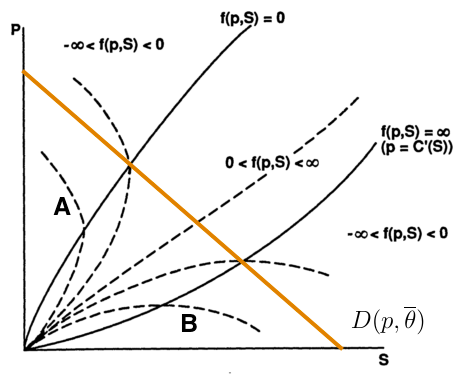
\includegraphics[width=8cm]{figintro/KMboundaries.png}
\caption{\small{This graph is adapted from the original paper by Klemperer and Meyer and illustrates the admissible region of solutions to the differential equation so as to verify the constraints on the slope of the supply function.}}
\label{KMboundaries}
\end{figure}

Therefore, the admissible set of solutions is defined by the upper bound of the demand shocks $\overline{\theta}$, in that if the solutions cross the slope boundaries before reaching the maximal shock, they cannot be accepted as solutions to the problem which constrains the solutions more strictly than the differential equation alone. In figure \ref{KMboundaries} the demand associated with the upper bound of the shocks $D(p,\overline{\theta})$ is represented in orange, and solutions A and B to the differential equation are not solutions to the problem as they reach the boundaries for smaller values of shocks.\\

The last result we will review here, is that in the case of an unbounded support of shocks, the set of equilibria is at its smallest, as it means that solutions have to have positive finite slope for every value of the shocks, and not only for a segment of the real line. \\

In some cases, for example for linear demand schedules, this set can collapse to a unique solution. \\

\subsection*{The case for ramping costs}

This framework models the costs as depending only on the quantity produced. In the context of electricity generation, an important type of costs that cannot be captured in such a specification of the cost function is that of ramping costs. These ramping costs refer to the fact that making production change over time induces specific costs.\\

To explain how such costs can arise, consider a thermal power plant (fossil fuels, nuclear etc.), and more precisely its core. Physically, to produce a given level of electricity, one has to maintain the core at a given temperature. To increase production, the temperature of the core has to increase. This means that when production is increased some fuel has to be lost to simply increase the temperature, this energy expenditure is not attached to any additional production.\\

This issue of ramping costs is at the heart of the choice of "quick" gas power plants to match sudden peaks in demand, where nuclear plants are more generally used for low frequency adjustments. Therefore these ramping costs are important technically on the electricity market. They are important enough for the project of European Power Exchanges named ``Price Coupling of Regions'' (PCR), which aims to develop a single price coupling solution to be used to calculate electricity prices across Europe, to consider the possibility to use load gradient orders, that is orders that condition their availability on the change in production from one hour to the next. However, at the moment of writing, PCR is still very much a work in progress \cite{EPEXPCR}.\\

Some papers have tried to estimate their values empirically, \cite{wolak2007quantifying} and more recently \cite{reguant2011welfare}. There is also a strand of litterature concerned with ramping costs, looking at the optimal price that allows to maximize the overall social welfare \cite{tanaka2006real}, that is, which price schedule allows to maximize the consumer welfare from which the production costs are substracted. This litterature does not use game-theoretical frameworks, but concerns itself with the best price signal to use in order to limit the ramping costs incurred due to varying demand, while still considering that the trajectory of demand is known. To our knowledge, there is no game-theoretical framework that has been brought to take ramping costs into account, and describe their effects on optimal strategies for the agents bidding on the market. 

\subsection*{Contribution}

This thesis focuses on the question of these ramping costs. In the first chapter, I tackle this question in a theoretical framework which yields predictions on the change of shape in supply functions over time as a function of the underlying uncertainty about demand shocks. The second chapter then introduces methods to study the shape of supply functions as observed on the French electricity market for data from 2011 to 2013, as well as methods to estimate the uncertainty contributed by the weather. The third chapter applies these methods to test these theoretical predictions on actual market data. The second and third chapters have been co-written with Henri de Belsunce, who finished his PhD in 2015 at the Munich-based Max Planck Institute for Innovation and Competition, under the supervision of Prof. Dr. Klaus M. Schmidt.\\

The first chapter focuses on what the introduction of ramping costs in a theoretical framework brings to the table. Our main contribution is to build and justify how these ramping costs can be tackled theoretically. First, we note that going to a continuous time descritption of the problem allows us to bring to the litterature about supply function equilibria powerful mathematical tools mostly used in option pricing, that is stochastic dynamics: we want to model ramping costs, i.e. costs associated to the variation in production, while retaining the key ingredient brought by \cite{KM}, i.e. the uncertainty, through the use of brownians, and more precisely, It\={o} processes. In so doing we face the issue that one cannot derive a brownian, and bring our second contribution, a physical argument about how power plants function that effectively operates as a low pass filter on our stochastic processes, and allow us to continue to build a tractable model of ramping costs under uncertainty. Third, we find in the litterature a specification of It\={o} processes that allows the model to remain tractable. \\

From these technical contributions we obtain our economic contributions in having a rich tractable model that yields results that contrast strongly with past results from the litterature. First, our solutions are unique, which contrasts with the usual continuum of Nash equilibria in the supply function equilibria litterature. Second, our solutions are not ex-post optimal, meaning that gathering information about the expected future evolution of demand yields different optimal strategies for suppliers, which in turn means that producers in our framework have a motive for submitting different supply functions from one time step to the next. Third, we have closed form solutions which yield specific predictions about the evolution of bids under uncertainty, namely that when uncertainty increase, suppliers submit steeper supply schedules in order to transmit more of these shocks to changes in price and not quantities, which are costly due to the existence of ramping costs. Finally, and less importantly, our framework justifies the existence of negative prices \footnote{Note that such negative prices happen, a few hours a year for example in France or Germany, for example in 2017 there were 146 such hours on 24 days in Germany \cite{epexnegP}} by producers being willing to pay consumers to consume more in order to avoid facing large variations in production, in contrast to everywhere positive schedules in the case of the supply function equilibria litterature. These results open the door to models being able to differentiate between day-ahead and intraday markets and therefore to offer a framework in which their interactions might be possible.\\

In the rest of the thesis the goal is to test our predictions on data from the French day-ahead market. In so doing, as our theoretical predictions are mainly about the effect that the amount of uncertainty has on the slope of the optimal supply schedule, we separate the issue of building proxies for this uncertainty in our second chapter, and the actual analysis of the evolution of bids on these proxies in the third chapter.\\

In the second chapter our main focus is on analyzing our data, on building a way to describe it, and on building proxies for the uncertainty that producers face about the residual demand they have to anticipate when bidding on the day-ahead market. \\

First, we note that aggregate supply functions on the day ahead market cannot be well captured by parametric functions. Therefore we devise a way to describe them non-parametrically: we note that although they cannot be captured parametrically, they still have a rough S shape, and therefore four main parts, two extremal sections, and two interior ones separated by the inflection point of the curve in its middle secion. We define the transition points between these sections as the points of maximal absolute value for the derivative and second derivative of the supply schedules. This definition relies on kernel density estimates, and is therefore non-parametric. We observe that by using 5 such points, we are able to capture about 98\% of the intrisic variability of the supply schedules, and stop there although our method can be used to define more non parametric points. This method allows us to define points that we consider comparable across auctions, that allow use to perform cross-sectional analysis of our data in the third chapter. \\

Second, we build proxies for the amount of weather uncertainty that producers face and variables that capture information that suppliers have before bidding and should therefore be controlled for. For the information available to suppliers, we note that the effect of weather on the demand, and more importantly temperature, is well understood and that we need to control for it. To do so we build an effective temperature for France, as an average of the localised temperature weighted by the population of the spatial region considered, in order to capture the overall effect temperature has on heating.\footnote{France has a high level of electric heating overall, which means that demand for electricity is quite sensitive to temperature.} The rest of our focus is on building a proxy for the uncertainty concerning renewable production. To do so we analyze spatialized wind and sunlight data, and study it's spatial structure. We argue that spatial autocorrelation is a proxy for the uncertainty associated with weather forecasts, noting that if this data displays more spatial gradients, it is likely to be of a lesser quality due to the numerical nature of the weather simulations used to predict the weather, and therefore more uncertain.\\

Our contribution in the second chapter is to provide a non parametric way to define comparable points across auctions, and a measure of the uncertainty associated with weather forecasts.\\

In the third chapter, we focus on building the main proxy for the uncertainty faced by producers, and then on analyzing how the bids evolve relative to these proxies.\\

We note that the main uncertainty is about the shape of the demand schedules itself. Therefore we consider data available to the producers and regress the demand schedules on these variables. Next, we study the residuals of these regressions, and more specifically note that they are heteroskedastic. We leverage this, regressing the square of these residuals on our variables, in order to predict the expected amplitude of the residuals, that is the amplitude of the uncertainty of the demand schedule regression.\\

We then study the effect of our different proxies for uncertainty on the slope of the supply schedules, and note that if our proxies about the weather uncertainty (through the channel of renewable production) have the expected effect, the results are less clear cut for our residuals on the demand schedules. As we are working with full blown schedules in the quantity-price plane, we perform our residual analysis both on the prices and the quantities. We therefore obtain estimates for the uncertainty pertaining to the position of a given point of our demand schedule either in price or in quantity. In our theoretical framework, we make the strong assumptions that demand schedules are linear, and that demand shocks are additive, i.e. they do not impact the slope of the demand schedules. These assumptions yield that we cannot differentiate between shocks in price or quantity, and that they should have effects in the same direction: more uncertainty implying steeper supply curves to reduce the amount of fluctuations in production. However we observe that the effects of price and quantity uncertainty as estimated by our residuals' method yield opposite effects. Both of these assumptions, although required to obtain closed form results, are clearly not satisfied by our data, and we think that this is a clear path for improvement of the model.  \\

The contribution of the third chapter is to provide a way to estimate the uncertainty about the demand schedules faced by suppliers, and to estimate how this uncertainty affects the shape of the supply schedules at different points along its overall length, i.e. we provide a framework to describe how the functional form of schedules is affected by estimates of the uncertainty faced by suppliers.

\newpage
\section*{Introduction Générale}
\subsection*{Évolution de la modélisation des marchés de l'électricité}
\subsubsection*{Tarification des services publics}

L'intérêt pour la modélisation des marchés de l'électricité remonte aux travaux de référence de Marcel Boiteux, vice-président en charge des études économiques d'EDF au sortir de la seconde guerre mondiale. La question principale à l'époque est celle de la tarification d'un service public : dans le contexte d'un monopole d'état, à quel prix les consommateurs devraient-ils faire face afin que les producteurs recouvrent leurs coûts. \\

Les producteurs d'électricité font face à deux contraintes particulières : le caractère incertain de la demande ainsi que sa périodicité, le tout pour un bien qui ne peut essentiellement pas être stocké.\footnote{Il est possible de stocker de l'électricité grâce à des barrages, mais l'énergie totale ainsi stockable n'est pas suffisante pour complètement stabiliser la demande à laquelle les moyens de production font face. Par ailleurs, seule une fraction de l'énergie ainsi stockée est renouvelable volontairement: les stations de transfert d'énergie par pompage disposent de deux lacs ce qui permet de pomper de l'eau d'un lac situé en aval vers un lac en amont et ainsi de reconstruire les réserves plus rapidement qu'en attendant que les affluents naturels du lac amont ne le remplissent.}\\

La première contrainte est traitée dans \cite{boiteux1951tarification}. Dans cet article, Boiteux considère une demande constante en moyenne mais sujette à des fluctuations. L'objectif est de trouver la tarification marginale permettant au consommateur d'internaliser le coût supplémentaire qu'une demande incertaine fait peser sur le producteur. Étant donné une certaine probabilité que la demande soit au dessus de sa valeur espérée d'une certaine quantité, il s'agit de trouver quelle capacité de reserve doit être maintenue en ligne pour garantir une probabilité cible de défaillance. \footnote{Dans le contexte de l'électricité, comme la production doit être égale à la demande à chaque instant, chaque réseau national est dimensionné avec un niveau de probabilité de défaillance acceptable. }\\

La seconde contrainte est traitée dans \cite{boiteux1960peak}. Contrairement à la situation précédente, la demande est ici considérée comme périodique et déterministe. L'objectif est de trouver la tarification permettant de transmettre aux consommateurs le coût d'investissement supplémentaire associé à une demande présentant des pics plus élevés.\\

Ces contributions nourrissent une large littérature sur la question de la tarification de biens non stockables faisant face à une demande cyclique, tout d'abord par \cite{brown1969public} qui étudie l'impact d'une demande stochastique sur le bien-être social espéré. Nous renvoyons la lectrice intéressée à la revue de littérature suivante: \cite{crew1995theory}.\\

Cette branche de la littérature se concentre principalement sur la question de la tarification optimale lorsque l'agent fixant le prix a pour objectif de maximiser le bien-être des consommateurs, dans le cas de monopoles d'état.\\

\subsubsection*{Évolutions de la régulation}
Cette branche de la littérature prend pour hypothèse que ces biens sont produits par des monopoles d'état. Il est alors admis que les services de réseau, comme le gaz, l'électricité ou les télécoms doivent être organisés sous la forme de monopoles verticalement intégrés.\\

Cette position évolue dans les années quatre-vingts, avec l'ouverture à la compétition de ces monopoles d'état. En 1984, l'accès aux gazoducs est ouvert à la compétition aux États-Unis et en 1990, la Grande-Bretagne privatise la fourniture d'électricité, en séparant production et transmission. Il est alors considéré que la condition de monopole naturel est liée au réseau, et qu'en séparant production et transmission, la production peut s'ouvrir à la compétition.\\

L'argument général en faveur de la libéralisation est que la compétition privée est considérée comme une voie plus sûre vers l'efficacité économique que la régulation d'un monopole. Dans une situation de compétition parfaite, les agents seraient ainsi fortement incité à rechercher des gains d'efficacité, et ces gains seraient transmis aux consommateurs \cite{schmidt1996costs}. La compétition parfaite étant une situation rare, une nouvelle branche de la littérature émerge autour de la question de la modélisation de la compétition dans le marché de l'électricité \cite{newbery1997privatisation}. \\

Bien que ce mouvement de libéralisation soit considéré comme permettant à minima des gains d'efficacité modestes à moyen terme \cite{fabrizio2007markets}, il ralentit après la crise californienne du début des années 2000 \cite{jamasb2005electricity}, qui se concentre principalement sur les marchés de gros de l'électricité. De très grandes fluctuations de prix ainsi que des pénuries ont lieu, principalement induites par une très faible elasticité-prix de la demande, ainsi que l'interaction entre le marché de gros et les contrats à terme \cite{borenstein2002trouble}. En Europe, la commission européenne pousse avec succès pour la poursuite du programme de libéralisation et d'intégration européenne, et les marchés de gros de l'électricité sont maintenant répandus sur le continent, sans que ne se produise de défaillances semblables à celles observées en Californie. 

\subsubsection*{Les marchés de l'électricité}
L'organisation des marchés de l'électricité est très fortement induite par deux caractéristiques importantes:
\begin{itemize}
\item Le marché se doit de refléter les changements rapides de demande.
\item La forme des enchères doit leur permettre de se satisfaire de la nature incertainte de la demande au moment de l'enchère.
\end{itemize}

Ces ingrédients sont à la source de la construction de marchés horaires voire même demi-horaires, au sein desquels les producteurs doivent soumettre des courbes d'offre pour un nombre déterminé d'enchères (en général uns fois par jour, soit 24 ou 48 courbes d'offre à la fois selon que l'enchère est horaire ou demi-horaire). Ces courbes d'offres prennent la forme d'un ensemble de paires de prix et de quantités monotone, qui peuvent définir des fonctions constantes par morceaux \footnote{comme dans le cas du marché de gros d'Angletterre et du Pays de Galles dans les années quatre-vingt-dix} ou des fonctions linéaires par morceaux. \footnote{les paires prix quantité sont considérées comme étant reliées par des linéaires, comme dans le cas du marché day-ahead français, mais aussi le marché anglais actuel (demi-horaire). Ces deux marchés spot sont gérés par la bourse EPEX Spot.}\\

Dans les années quatre-vingts, une impulsion théorique cherche à modéliser ces marchés sous forme d'équilibres en courbes d'offres. Cette approche est introduite en premier lieu par \cite{grossman1981nash} and \cite{hart1982imperfect}. Ils considèrent une situation où des producteurs rivalisent via des courbes d'offres en faisant face à une courbe de demande connue et donnée. Le princpal résultat de cette approche est que ces modèles peuvent être résolus, que les stratégies optimales en courbe d'offre peuvent être spécifiées, mais qu'il existe un forte multiplicité d'équilibre dans ce contexte.\\

Peu de temps après, \cite{klemperer1986price} introduisent un modèle dans lequel les producteurs choisissent d'entrer en concurrence en prix ou en quantité de façon endogène. Cette approche donne également lieu à une grande multiplicité d'équilibre, mais le résultat clef est que cette multiplicité est drastiquement réduite lorsque de l'incertitude est introduite dans le modèle.\\

Ce résultat inspire le papier fondateur \cite{KM} qui étudie une situation de compétition en courbes d'offres face à une demande incertaint. Dans cet article, bien qu'il y ait toujours un continuum d'équilibres, ce continuum possède une structure qui peut être étudiée lorsque la demande est incertaine. Dans le reste de cette thèse, nous appelons les équilibres en courbes d'offre des SFE (supply function equilibria).\\

Le modèle général proposé par Klemperer et Meyer est rapidement mis à profit pour décrire les marchés de l'électricité, la compétition sur le marché spot anglais est ainsi étudiée avec des SFE par \cite{Newgreen}.\\

Cet usage des SFE déclenche des débats sur la validité qu'il y a à décrire le marché de l'électricité, à l'époque encore principalement caractérisé par des enchères constantes par morceaux, avec des fonctions continues et dérivables : \cite{von1993spot} présente un argument montrant qu'une compétition via des constantes par morceaux de tailles finies exhibe des comportements fondamentalement différents du cas de fonctions continues. \footnote{Ce débat est principalement obsolète maintenant que la plupart des marchés sont passés à des linéaires par morceaux et plus des constantes par morceaux.} Des résultats empiriques montrent également que les stratégies prédites par cette classe de modèles diffèrent de façon significative des stratégies effectivement observées sur les marchés, voir \cite{willems2009cournot} et \cite{willems2009cournot}. Ces résultats interrogent sur la validité de l'approche SFE pour décrire les marchés de l'électricité, plus précisément la question est de savoir si les modèles de SFE sont valides mais attendent d'être perfectionnés, par exemple en les modélisant explicitement sous la forme de fonctions affines par morceaux \cite{baldick2004theory}, ou si cette approche est fondamentalement incapable de capturer les stratégies observées.\\

Cette approche est toutefois encore considérée comme pertinente par nombre d'auteurs, bien que la multiplicité des équilibres complique l'analyse des résultats théoriques. Par ailleurs les solutions ne sont pas directement exploitables, étant définies implicitement comme solution d'équations différentielles, et donc sans forme analytique dans la majorité des cas. Pour dépasser ces limites, la littérature cherche à décrire la compétition dans des cadres plus simples, par exemple dans des modèles de compétition de Cournot appliquée au cas des marchés de l'électricité dans le cas de \cite{borenstein1999empirical}, ou choisissent de se restreindre à une solution particulière parmi le continuum de solutions obtenu dans un contexte de SFE: l'unique solution linéaire du lot. Ces auteurs choisissent donc arbitrairement une solution tractable et s'en servent pour pousser le raisonnement économique plus loin qu'habituellement possible en conservant le continuum de solutions. \`A titre d'exemple, \cite{green1996increasing} se focalise sur la courbe d'offre linéaire parmi le continuum obtenu dans le cadre des SFE et se sert de son expression analytique pour étudier les effets de trois politiques d'encadrement de la compétition, quand \cite{hobbs2000strategic} fait de même pour étudier les contraintes de transmission. \\

Par ailleurs, il est important de noter que les marchés day-ahead n'existent pas hors-sol, et que l'électricité peut être echangée sur ces marchés mais aussi par des contrats à terme ou encore sur les marchés intraday. Il existe aussi des marchés de capacité ou une garatie de capacité disponible à une certaine date s'échange. Tous ces marchés interagissent les uns avec les autres, et une partie de la littérature s'attache à décrire ces interactions. Les SFE utilisés à cette fin sont généralement simplifiés, par exemple en ne considérant que les équilibres linéaires pour étudier l'interaction entre marché day-ahead et contrats à terme \cite{green1999electricity}, ou encore en considérant des équilibres assymétriques linéaires dans le même but \cite{anderson2012asymmetric}. Ces articles se concentrent généralement sur les interactions entre contrats à terme et marché day-ahead car les SFE ne sont pas en mesure de distinguer le marché day-ahead du marché intraday.\\

Nous renvoyons la lectrice intéressée vers la revue de littérature \cite{ventosa2005electricity} pour une vue d'ensemble plus détaillés. Dans cette thèse nous nous appuyons fortement sur le travail de Klemperer et Meyer, et contrastons souvent nos résultats aux leurs. Pour faciliter la lecture au lecteur qui ne serait pas familier avec leurs travaux, nous résumons ci-après leurs résultats sur lesquels nous nous appuyons. 

\subsection*{Klemperer et Meyer 1989}
Soit un marché sur lequel des producteurs enchérissent des courbes d'offre tout en faisant face à une demande incertaine.\\

Soit $D(p,\theta)$ la courbe de demande comme fonction du prix $p$ et du choc $\theta$. Considérons que pour tout $(p,\theta)$, $-\infty<D_p<0$, $D_{pp}\leq 0$ et $D_\theta>0$.\\

Les producteurs font face à la même fonction de coût $C(\cdot)$, avec $C'(q)>0$ et $0<C''(q)<\infty$ pour tout $q>0$.\\

Les producteurs soumettent leurs offres en même temps avant la réalisation du choc de demande $\theta$. Considérons pour l'instant deux producteurs $i$ et $j$ avec $S^k(p)$ la courbe d'offre du producteur $k$ différentiable deux fois. Une fois le choc connu, chaque producteur produit la quantité $S^k(p^*(\theta))$ au prix $p^*(\theta)$, tel que $D(p^*(\theta)) = S^i(p^*(\theta)) + S^j(p^*(\theta))$.\\

La demande résiduelle du producteur $i$ est donnée par la demande totale à  laquelle la production du producteur $j$ est soustraite, $D(p,\theta) - S^j(p)$. Comme $\theta$ est un scalaire, l'ensemble de points maximisant le profit pour chaque choc $\theta$ possible définit une courbe. Si il existe une intersection unique entre la courbe d'offre de $i$ et toute courbe de demande possible, alors cette courbe d'offre est ex-post optimale, c'est à dire qu'elle est optimale point à point pour chaque réalisation possible de $\theta$. \\

Sous l'hypothèse que les courbes d'offres se comportent effectivement de cette manière, la maximisation du profit espéré devient indépendante de la distribution des chocs de demande, et la courbe d'offre optimale de $i$ résout pour chaque choc $\theta$ le programme de maximisation suivant :

\begin{equation}\label{maxKMfr}
\max_p p\left( D(p,\theta) - S^j(p)\right) - C\left( D(p,\theta) - S^j(p)\right) 
\end{equation}

dont la condition du premier ordre s'écrit :

\begin{equation}\label{KMfocfr}
\ D(p,\theta) - S^j(p) + \left( p - C^\prime\left( D(p,\theta) - S^j(p)\right)    \right)\left(  D_p(p,\theta)   - S^{j\prime}(p)\right) = 0
\end{equation}

Comme l'équation \ref{maxKMfr} est strictement concave en $p$ (nous renvoyons le lecteur vers le papier original pour plus de détails), l'équation \ref{KMfocfr} définit un unique prix $p^*(\theta)$ maximisant le profit pour chaque choc $\theta$, qui paramétrise la courbe d'offre optimale. \\

Considérons que $D_{\theta p }=0$, c'est à dire que $\theta$ est un choc additif, et concentrons nous sur les équilibres symmétriques, ce qui nous permet de ne plus faire attention aux exposants $i$ et $j$ caractérisant la productrice. Sachant que l'eq. \ref{KMfocfr} doit être vérifiée pour tout choc, elle peut se réécrire :

\begin{equation}\label{KMdifffr}
S'(p) = \frac{S(p)}{p-C'(S(p))} + D_p(p)= f(p,S)
\end{equation}
Cette équation différentielle définit l'équilibre en courbes d'offres, l'incertitude ayant pour conséquence que cette équation doit être vérifiée pour tout choc, et donc pour tout prix possible. Cette équation ne s'accompagne toutefois pas d'une condition initiale. Il existe donc une multiplicité de solutions admissibles.\\

Les courbes d'offres sont bornées par les possibles valeurs de leur pente, qui doit être comprise entre $0$ et $+\infty$. Il est possible de définir le lieu des points pour lesquels les solutions de l'équation différentielle ont pour pente ces valeurs extrémales, qui définit donc la région des solutions admissibles dans notre contexte : 

\begin{figure}[h]
\centering
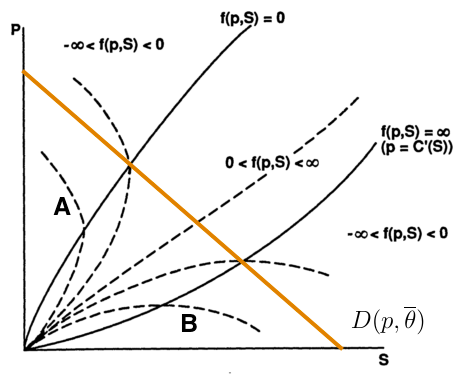
\includegraphics[width=8cm]{figintro/KMboundaries.png}
\caption{\small{Ce graphique est adapté du papier orginal de Klemperer et Meyer et illustre la region de solutions de l'équation différentielle admissibles dans le cadre de notre problème, c'est à dire vérifiant les contraintes sur leur pente.}}
\label{KMboundariesfr}
\end{figure}

L'ensemble des solutions admissibles est donc définit par la borne supérieure de nos chocs de demande $\overline{\theta}$, en cela que si une solution de l'équation différentielle devait traverser les frontières définies ci dessus pour un choc inférieur au choc maximal, elle ne serait pas pour autant solution de notre problème qui contraint plus fortement les solutions que l'équation différentielle seule. Dans la figure \ref{KMboundariesfr}, la demande associée avec le choc maximal $D(p,\overline{\theta})$ est représenté en orange et les solutions A et B de l'équation différentielle ne sont pas solution de notre problème car elles franchissent nos frontières pour des valeurs de chocs inférieures à ce maximum.\\

Le dernier résultat que nous évoquerons ici est que dans le cas d'un support de choc infini, l'ensemble d'équilibres symmétriques est le plus petit possible, car il faut dans ce cas que toute solution ait une pente positive et finie pour tout choc positif et plus seulement pour un segment de la droite des réels.\\

Dans certains cas, par exemple pour des courbes de demande linéaires, cet ensemble peut converger vers une solution unique.\\

\subsection*{Les coûts de variation}

Ce modèle choisit de considérer des coûts ne dépendant que de la quantité produite. Dans le contexte de la production d'électricité, il existe un type de coûts qui ne peut pas se modéliser ainsi, les coûts de variation. Ces coûts sont induits lorsque la production varie dans le temps.\\

Afin d'expliquer ces coûts, considérons une centrale thermique (fossile, nucléaire etc.) et plus précisémment son réacteur. Physiquement, pour produire une certaine puissance, il faut maintenir le réacteur à une température donnée. Afin d'accroître la production, la température du réacteur doit augmenter. Cela implique que lorsque la production augmente, du combustible doit être perdu afin de simplement réchauffer le réacteur, cette dépense énergétique n'étant pas associée à une production d'énergie. \\

L'existence de ces coûts est au coeur du choix d'utiliser des centrales gaz "rapides" afin de suivre une hausse soudaine de la demande, là où les centrales nucléaires sont plus généralement utilisées afin de suivre les changements basse fréquence de la demande. Ces coûts sont suffisamment importants pour que le projet des bourses européennes d'électricité EPEX intitulé ``Price Coupling of Regions'' (PCR), qui cherche à développer un unique mécanisme de couplage des prix européens de l'électricité, considère la possibilité de soumettre des ordres conditionnés sur les gradients de chargem c'est à dire des ordres dont la disponibilité serait conditionnée sur le respect de valeurs maximales de variation de la production d'une enchère à l'autre. Le projet PCR n'est toutefois qu'à l'était d'ébauche au moment de l'écriture de ces lignes \cite{EPEXPCR}.\\

Des articles se sont attachés à estimer la valeur de ces coûts de variation empiriquement, \cite{wolak2007quantifying} et plus récemment \cite{reguant2011welfare}. Il existe également une branche de la littérature s'intéressant à ces coûts à travers le prisme de leur impact sur le prix optimal maximisant le bien-être social \cite{tanaka2006real}, c'est à dire s'intéressant à la chronique temporelle de prix permettant de maximiser l'utilité des consommateurs à laquelle sont soustraits les coûts de variation. Ces travaux ne s'inscrivent pas dans une approche de théorie des jeux, mais cherchent à trouver le signal prix permettant de limiter les coûts de variation induits par une demande variant de façon déterministe. \`A notre connaissance il n'existe pas de modèle de ces coûts dans un contexte de théorie des jeux permettant de décrire leur impact sur les stratégies optimales des producteurs jouant sur le marché de l'électricité.

\subsection*{Contribution}
Cette thèse se concentre sur la question des coûts de variation. Dans le premier chapitre cette question est abordée dans un modèle théorique produisant des prédictions sur l'évolution de la forme des courbes d'offres optimales dans le temps en fonction de la dynamique sous-jacente des chocs de demande. Le deuxième chapitre introduit ensuite des techniques permettant d'étudier empiriquement la forme des courbes d'offre observées sur le marché de l'électricité français entre 2011 et 2013, ainsi que des méthodes permettant d'estimer l'incertitude sur la demande associée à la météo. Le troisième chapitre applique ces méthodes afin de tester empiriquement les prédictions théoriques du premier chapitre. Ces deux derniers chapitres sont issus d'une collaboration avec Henri de Belsunce, qui a soutenu son doctorat en 2015 au Max Planck Institute for Innovation and Competition de Munich, sous la supervision de Prof. Klaus M. Schmidt.\\

Le premier chapitre se concentre sur ce que la prise en compte des coûts de variation apporte dans un contexte théorique. La contribution principale est de contruire et de justifier comment tenir compte théoriquement des ces coûts. En premier lieu, nous passons à une description du problème en temps continu afin d'apporter a la littérature sur les SFE des outils mathématiques puissants surtout utilisés en finance, à savoir la dynamique stochastique : nous cherchons en effet à modéliser les coûts de variation, en conservant l'ingrédient clef introduit par \cite{KM}, i.e. l'incertitude, grâce à l'utilisation de browniens, plus précisémment des processus d'It\={o}. Ce faisant, nous faisons face au caractère non dérivable des processus stochastiques, et apportons notre deuxième contribution, un argument physique concernant la mode de fonctionnement des centrales de production qui opèrent effectivement comme des filtres passe-bas sur nos processus stochastiques et qui nous permet de continuer à construire un modèle tractable de coûts de variation avec incertitude. Troisièmement, nous trouvons une spécification d'un processus d'It\={o} nous permettant de conserver un forme analytique. \\

De ces contributions techniques nous obtenons nos contributions économiques grâce à un modèle riche et tractable qui propose des résultats contrastant fortement avec les résultats passés de la littérature. Tout d'abord, nos solutions sont uniques, contrairement aux continuums d'équilibres de Nash habituels dans la littérature des SFE. Deuxièmement, nos solutions ne sont pas ex-post optimales, c'est à dire qu'acquérir de l'information sur l'evolution attendue de la demande induit des stratégies optimales différentes pour les producteurs, ce qui a pour conséquence que les producteurs dans notre modèle ont une justification pour soumettre des enchères variant dans le temps. Troisièmement, nous obtenons des formes analytiques faisant des prédictions précises sur l'évolution des stratégies avec la dynamique des chocs de demande, à savoir que lorsque l'incertitude sur la demande augmente, les producteurs soumettent des courbes d'offre de plus en plus pentues afin de transmettre une plus grande part des chocs de demande aux prix plutôt qu'aux quantités dont les variations sont coûteuses. Enfin, notre modèle justifie l'existence de prix négatifs\footnote{De tels prix négatifs s'observent sur les marchés de l'électricité quelques heures par an en moyenne pour l'Allemagne et la France, par exemple en 2017 il y a eu 146 heures en Allemagne pour lesquelles les prix étaient négatifs, répartis sur 24 jours \cite{epexnegP}} avec des producteurs étant prêts à subventionner la demande pour ne pas avoir à faire face de forts coûts de variation, ce qui contraste avec les courbes d'offre partout positives dans les modèles de SFE. Ces résultats ouvrent la porte à des modèles capables de différencier entre marchés day-ahead et intraday et donc potentiellement de modéliser leurs interactions.\\

Dans le reste de la thèse l'objectif est de tester ces prédictions sur des donnés issues du marché day-ahead français. Comme ces prédictions portent avant tout sur l'impact de l'incertitude sur la forme des courbes d'offre, nous séparons en deux chapitre la contruction de proxys pour cette incertitude dqns le deuxième chapitre et l'analyse de l'évolution des enchères en fonction de cette incertitude dans le troisième chapitre.\\

Dans le second chapitre nous nous concentrons sur l'analyse de nos données, sur le développement d'une méthodologie permettant d'utiliser des données dont chaque observation est une fonction, et sur la construction de proxys pour l'incertitude à laquelle les producteurs font face vis à vis de la demande résiduelle qu'ils se doivent d'anticiper lorsqu'ils jouents leurs enchères sur le marché day-ahead.\\

Nous notons d'abord que les courbes d'offre agrégées sur le marché day-ahead ne sont pas bien capturées par des fonctions paramétriques. Nous construisons une approche non paramétrique pour les décrire : nous notons que malgré leur mauvaise approximation par des fonctions paramétriques elles sont néanmoins grossièrement en forme de S, et donc constituées de quatre grandes parties, les deux sections extrémales, et deux sections intérieures séparées par le point d'inflexion de la fonction. Nous définissons les points de transition entre ces sections comme étant les points pour lesquels les valeurs absolues des premières et secondes dérivées de nos courbes d'offres sont maximales. Cette définition repose sur des estimations de densité de kernels, et est donc bien non paramétrique. Nous remarquons qu'en utilisant 5 de ces points, nous sommes en mesure de capturer environ 98\% de la variabilité intrinsèque des courbes d'offre, et nous contentons donc de ces 5 points bien que notre méthode peut servir à définir plus de points. Cette méthode nous permet de caractériser des points que nous considérons comparables d'une enchère à l'autre et nous permet de réaliser l'analyse de nos données dans le chapitre 3.\\

Nous construisons ensuite des proxys pour le degré d'incertitude associée à la météo à laquelle les producteurs doivent faire face ainsi que des variables capturant l'information disponible aux producteurs avant les enchères et que nous devons contrôler. La météo étant connue aux moment d'enchérir et ayant une influence sur la demande résiduelle, il nous faut en tenir compte. Néanmoins la météo influence la demande par des effets locaux là où le marché a lieu au niveau national, il nous faut donc construire des proxys nationaux des variables météo localisées sur le territoire français dont nous disposons. Nous construisons notamment un proxy national de température basé sur une moyenne de la météo localisée pondérée par la population afin de capturer l'effet de la température sur la demande à travers le chauffage notamment. \footnote{Une large proportion du chauffage en France est électrique, ce qui induit que la demande électrique en France est assez météo-sensible.} Le reste de notre travail consiste à construire des proxys pour l'incertitude concernant la production renouvelable qui vient réduire la demande résiduelle. Pour ce faire nous analysons la structure spatiale de nos données de vent et de rayonnement. Nous défendons le fait que l'autocorrélation spatiale de ces variables est un proxy de l'incertitude, en notant que plus les gradients spatiaux sont élevés, moins la prédiction météo sur laquelle se basent les producteurs au moment de jouer sur le marché sera de qualité.\\

Dans ce second chapitre nous développons une méthode non paramétrique permettant de comparer les observations fonctionnelles dont nous disposons les unes aux autres, ainsi que des proxys pour l'incertitude associée à la météo.\\

Dans le troisième chapitre, nous nous concentrons sur la construction du proxy principal pour l'incertitude à laquelle les producteurs font face, l'incertitude sur la courbe de demande agrégée, et nous attachons ensuite à décrire comment les enchères évoluent avec nos différentes sources d'incertitude.\\

Nous considérons les informations accessibles aux producteurs au moment d'enchérir et régressons les courbes de demandes sur ces variables. Nous étudions ensuite les résidus de cette régression et notons qu'ils sont hétéroskédastiques. Nous nous servons de cette propriété en regressant le carré de ces résidus sur nos variables explicatives, afin de prédire l'amplitude attendue de ces résidus, c'est à dire l'amplitude de l'incertitude sur la courbe de demande au moment d'enchérir.\\

Nous étudions ensuite l'effet de nos différentes sources d'incertitude sur la pente de nos courbes d'offre, et notons que nos proxy pour l'incertitude météo se comportent comme attendus selon nos résultats théoriques obtenus dans le premier chapitre, alors que les résultats sur l'incertitude associée aux courbes de demande sont moins tranchés. Comme nos courbes de demande sont des fonctions complètes dans le plan prix-quantité, nous réalisons l'analyse de nos résidus tant en prix qu'en quantité. Nous obtenons donc des estimations de l'incertitude associée à la position d'un point de nos courbes de demande en prix et en quantité. Dans notre modèle théorique, nous faisons des hypothèses fortes sur la forme de la demande, que nous supposons linéaire, et nous supposons que les chocs de demande sont additifs, i.e. ils ne changent pas la pente de la demande. Ces hypothèses ont pour conséquence qu'il est impossible de différencier l'impact d'une incertitude en prix ou en quantité, et que ces deux incertitudes devraient avoir des effets de même signe: plus d'incertitude induit une pente plus grande de la courbe d'offre pour réduire la variation de la production. Nous observons néanmoins que les effets estimés de l'incertitude sur la quantité et le prix sont de signe opposés. Ces deux hypothèses, bien que nécessaires pour obtenir des solutions analytiques, sont évidemment violées par nos donnés, et nous pensons qu'il s'agit d'une piste importante d'amélioration du modèle.\\

La contribution du dernier chapitre est de proposer une méthodologie estimant l'incertitude directe sur la courbe de demande et d'estimer comment cette incertitude impacte la forme des courbes d'offre en différents points de son graph, i.e. nous proposons une approche permettant d'estimer comment les courbes d'offre se déforment sous l'effet de l'incertitude.\\



 